% !TeX encoding = UTF-8
\chapter{Оформление приложений}
\label{app:1}

Оформление приложений начинается заданием команды \verb|\appendix|, которая изменяет стиль оформления документа. После данной команды, команда \verb|\chapter{Название}| задает не новые главы, а новые приложения, которые нумеруются буквами. Изменяется нумерация и у других элементов, таких как рисунки, таблицы и формулы, примеры которых приведены ниже (см. рисунок \ref{app:fig}, формулу (\ref{app:eq}) и таблицу \ref{app:tab}).

\begin{figure}[ht!]
\begin{center}
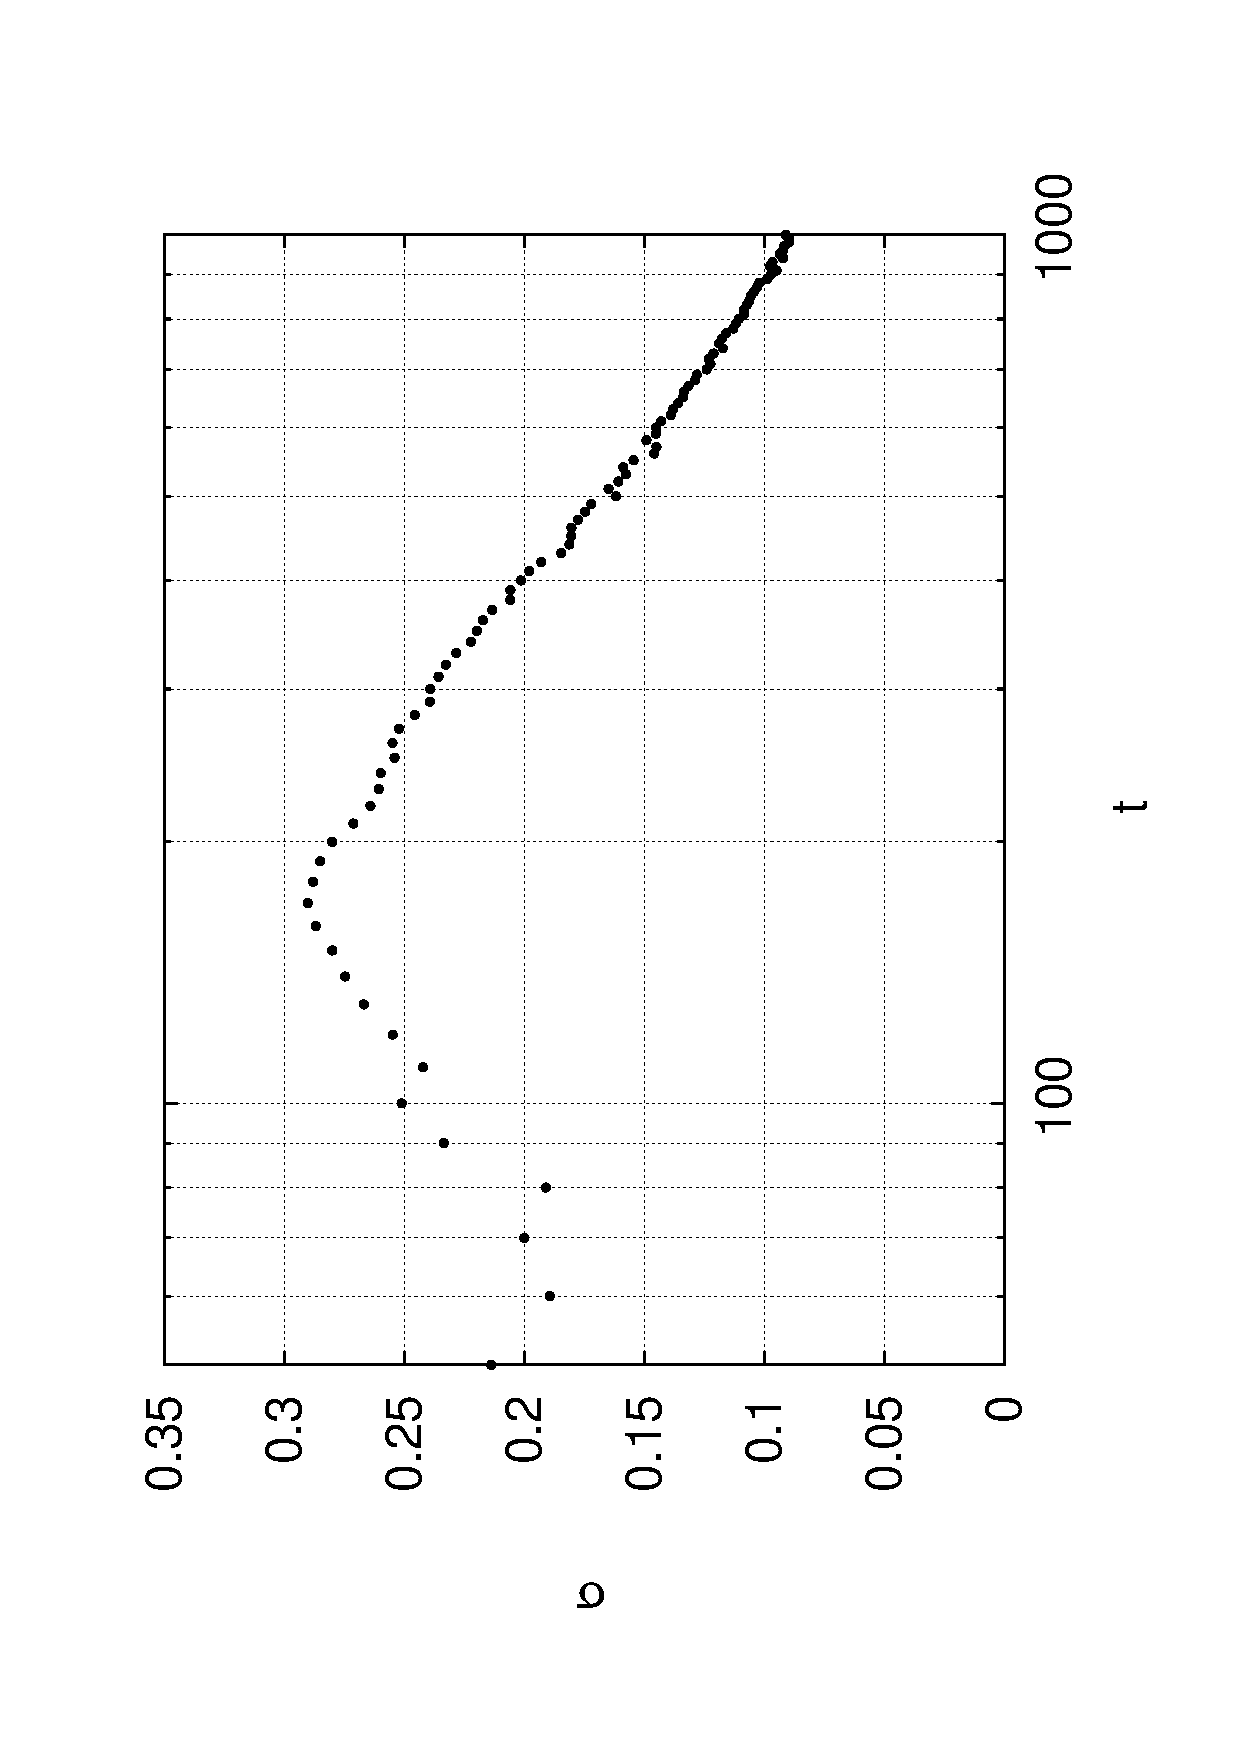
\includegraphics[angle=270,width=7cm]{test}\\
\caption{Подпись к рисунку. Дополнительная информация}
\label{app:fig}
\end{center}
\end{figure}

\begin{equation}\label{app:eq}
V = x^4 - 2 x^2,
\end{equation}
\begin{eqrem}
$x$ -- координата частицы.
\end{eqrem}

\begin{table}[h]
\caption{Характеристики процессов формирования волокон}
\begin{center}
\begin{tabular}{|>{\small}l|>{\small}c|>{\small}c|}
\hline
Наименование показателей & Вискоза & Камилон \\
\hline
Максимальная фильерная вытяжка, \% &12 &80\\
\hline
Температура осадительной ванны, \textcelsius &50 &20\\
\hline
Максимальная кратность вытягивания, \% &100 &30\\
\hline
\end{tabular}\label{app:tab}
\end{center}
\end{table}


\section{Раздел в приложении \ref{app:1}}

Приложение может разбиваться на разделы, подразделы и пункты с использованием стандартных команд секционирования.

\chapter{Сцепленные шаблоны диссертации, автореферата и презентации}\label{app:template}

Ниже представлена таблица \ref{table}, которая дает визуальное представление структуры сцепленных шаблонов диссертации, автореферата, презентации и списка вспомогательных файлов, которые включены в главные файлы через команду \verb|\include{имя файла}|.

Удобство использования сцепленных шаблонов заключаетсяв отсутсвии надобности дублировать одни и те же данные в разных документах. Например, положения выносимые на защиту должны дублироваться в диссертации, автореферате и презентации. Использование файла \textit{statements.tex}, которое содержит положения и используется во всех указанных выше документах, значительно упрощает работу над диссертацией и исключает необходимость постоянно следить за согласованностью положений в разных документах. То же касается частей диссертации, которые также должны быть и в автореферате (введение, общая характеристика работы, заключение и рекомендации по практическому использованию результатов).

\begin{table}[t]
\caption{Таблица, поясняющая структуру и связи в сцепленных шаблонах диссертации, автореферата и презентации}\label{table}
\begin{center}
\begin{tabular}{|p{58mm}|p{48mm}|p{49mm}|}
\hline
\large \bfseries ДИССЕРТАЦИЯ & \large \bfseries АВТОРЕФЕРАТ & \large \bfseries ПРЕЗЕНТАЦИЯ \\[2mm]
\hline
\multicolumn{3}{|c|}{\bfseries Главный файл}\\
\hline
\itshape THESIS.tex & \itshape ABSTRACT-PhD.tex & \itshape PRESENTATION.tex \\
\hline
\multicolumn{3}{|c|}{\bfseries Включенные файлы}\\
\hline
\multicolumn{3}{|c|}{\textit{statements.tex} -- положения, выносимые на защиту}\\
\hline
\multicolumn{3}{|p{16cm}|}{Рисунки хранятся в папке \textit{``fig''} в pdf формате. Обработка теховского файла производится pdfLaTeX. Для обычного LaTeXa нужны EPS рисунки.}\\
\hline
\textit{definitions.tex} -- список определений,
\newline \textit{titlepage.tex} -- титульная страница,
\newline \textit{thesisintro.tex} -- начало диссертации  &  \bfseries \large --- &
\textit{beamerthemeMinsk.sty} - стиль ``Минск'' для презентации (можно использовать любой другой стиль, см. \cite{beamer}) \\
\hline
\multicolumn{2}{|c|}{\textit{intro.tex} -- введение} & \bfseries \large --- \\
\hline
\multicolumn{2}{|c|}{\textit{characteristics.tex} -- общая характеристика работы} & \bfseries \large --- \\
\hline
\textit{chapter1.tex, chapter2.tex, chapter3.tex, chapter4.tex} -- четыре главы & \bfseries \large ---   & \bfseries \large --- \\
\hline
\multicolumn{2}{|c|}{\textit{conclusions.tex} -- заключение} & \bfseries \large --- \\
\hline
\multicolumn{2}{|p{11cm}|}{\textit{recommendations.tex} -- рекомендации по практическому использованию результатов} & \bfseries \large --- \\
\hline
\textit{bib.tex} -- библиографический список + статьи автора & \bfseries \large ---   & \bfseries \large --- \\
\hline
\multicolumn{2}{|p{11cm}|}{\textit{bibmypapers.tex} -- статьи соискателя в научных журналах} & \bfseries \large ---  \\
\hline
\multicolumn{2}{|p{11cm}|}{\textit{bibmyreports.tex} -- статьи соискателя в материалах конференций} & \bfseries \large ---  \\
\hline
\textit{appendix.tex} -- приложения.  & \bfseries \large ---   & \bfseries \large --- \\
\hline
\end{tabular}
\end{center}

\end{table}


\chapter{Нумерация приложений}

Согласно требованиям, приложения следует обозначать заглавными буквами русского алфавита. В данном классе это организуется автоматически при задании команды начала нового приложения \verb|\chapter{Название приложения}|. Но нужно обратить внимание на то, что не все буквы могут быть использованы для нумерации. Буквы Ё, З, Й, О, Ч, Ь, Ы, Ъ должны быть исключены из нумерации. В классе использована функция \verb|\Asbuk| для формы представления счетчика приложений, которая сама не включает в нумерацию буквы Ё, Й, Ь, Ы, Ъ. Но буквы З, О, Ч, остаются. Для их исключения перед приложением, которое может получить неподходящую букву, нужно изменить счетчик приложений {\itshape chapter}, используя команду \verb|\addtocounter{chapter}{1}|.

Для нумерации приложений также можно пользоваться буквами латинского алфавита. Для этого сразу после команды  \verb|\appendix|, задающей начало приложений, нужно переопределить форму командой: \verb|\renewcommand{\thechapter}{\Alph{chapter}}|. Исключение лишних букв I и O из нумерации осуществляется описанным выше способом.


\chapter{Таблица с больш\'{и}м количеством строк}
\label{app:table}

Ниже приведен пример таблицы с большим количеством строк. Основные объяснения по оформлению данного типа таблиц приведены в подразделе~\ref{sec:ltable} и книге \cite[раздел 12.5]{Kotelnikov}.

\begin{longtable}{|l|c|c|}
\caption{Подпись к таблице с большим количеством строк. Таблица занимает две страницы.}
\label{tab:long}
 \\ \hline
Боковик & Первый столбец & Второй столбец \\ \hline
		\endfirsthead
\multicolumn{3}{l}{Продолжение таблицы \ref{tab:long}}
\\ \hline
Боковик & Первый столбец & Второй столбец \\ \hline
		\endhead
		\endfoot
	\hline  \endlastfoot

Название & Элемент первого столбца & Элемент второго столбца \\
Название & Элемент первого столбца & Элемент второго столбца \\
Название & Элемент первого столбца & Элемент второго столбца \\
Название & Элемент первого столбца & Элемент второго столбца \\
Название & Элемент первого столбца & Элемент второго столбца \\
Название & Элемент первого столбца & Элемент второго столбца \\
Название & Элемент первого столбца & Элемент второго столбца \\
Название & Элемент первого столбца & Элемент второго столбца \\
Название & Элемент первого столбца & Элемент второго столбца \\
Название & Элемент первого столбца & Элемент второго столбца \\
Название & Элемент первого столбца & Элемент второго столбца \\
Название & Элемент первого столбца & Элемент второго столбца \\
Название & Элемент первого столбца & Элемент второго столбца \\
Название & Элемент первого столбца & Элемент второго столбца \\
Название & Элемент первого столбца & Элемент второго столбца \\
Название & Элемент первого столбца & Элемент второго столбца \\
Название & Элемент первого столбца & Элемент второго столбца \\
Название & Элемент первого столбца & Элемент второго столбца \\
Название & Элемент первого столбца & Элемент второго столбца \\
Название & Элемент первого столбца & Элемент второго столбца \\
Название & Элемент первого столбца & Элемент второго столбца \\
Название & Элемент первого столбца & Элемент второго столбца \\
Название & Элемент первого столбца & Элемент второго столбца \\
Название & Элемент первого столбца & Элемент второго столбца \\
Название & Элемент первого столбца & Элемент второго столбца \\
Название & Элемент первого столбца & Элемент второго столбца \\
Название & Элемент первого столбца & Элемент второго столбца \\
Название & Элемент первого столбца & Элемент второго столбца \\
Название & Элемент первого столбца & Элемент второго столбца \\
Название & Элемент первого столбца & Элемент второго столбца \\
Название & Элемент первого столбца & Элемент второго столбца \\
Название & Элемент первого столбца & Элемент второго столбца \\
Название & Элемент первого столбца & Элемент второго столбца \\
Название & Элемент первого столбца & Элемент второго столбца \\
Название & Элемент первого столбца & Элемент второго столбца \\
Название & Элемент первого столбца & Элемент второго столбца \\
Название & Элемент первого столбца & Элемент второго столбца \\
Название & Элемент первого столбца & Элемент второго столбца \\
Название & Элемент первого столбца & Элемент второго столбца \\
Название & Элемент первого столбца & Элемент второго столбца \\
Название & Элемент первого столбца & Элемент второго столбца \\
Название & Элемент первого столбца & Элемент второго столбца \\
\end{longtable}
%\end{table}

\chapter{Таблица с больш\'{и}м количеством столбцов}
\label{app:gtable}

Ниже приведен пример таблицы с большим количеством столбцов. Основные объяснения по оформлению данного типа таблиц приведены в подразделе~\ref{sec:gtable}.

\begin{table}[h]
\caption{Характеристики процессов формирования волокон из гидратцеллюлозы}
\label{tab:g}
\begin{tabular}{|>{\small}l|>{\small}c|>{\small}c|>{\small}c|}
\hline
Наименование показателей & Вискоза & Камилон & Волокно \textnumero 3 \\
\hline
Максимальная фильерная вытяжка, \% &12 &80 &42 \\
\hline
Температура осадительной ванны, \si{\celsius} &20 &12 &80 \\
\hline
Максимальная кратность вытягивания, \% &100 &32 &84 \\
\hline
\end{tabular}

\smallskip
Продолжение таблицы \ref{tab:g}\\
\begin{tabular}{|>{\small}l|>{\small}c|>{\small}c|>{\small}c|}
\hline
Наименование показателей & Волокно \textnumero 4 & Волокно \textnumero 5 & Волокно \textnumero 6 \\
\hline
Максимальная фильерная вытяжка, \% &80 &42 &83 \\
\hline
Температура осадительной ванны, \si{\celsius} &20 &12 &80 \\
\hline
Максимальная кратность вытягивания, \% &100 &32 &84 \\
\hline
\end{tabular}

\smallskip
Окончание таблицы \ref{tab:g}\\
\begin{tabular}{|>{\small}l|>{\small}c|>{\small}c|>{\small}c|}
\hline
Наименование показателей & Волокно \textnumero 7 & Волокно \textnumero 8 & Волокно \textnumero 9 \\
\hline
Максимальная фильерная вытяжка, \% &80 &42 &82 \\
\hline
Температура осадительной ванны, \si{\celsius} &40 &12 &80 \\
\hline
Максимальная кратность вытягивания, \% &100 &34 &84 \\
\hline
\end{tabular}


\end{table}


